%% \documentclass[compress,12pt]{beamer}

%% \usepackage{mathrsfs}
%% \usepackage{stmaryrd} % \llbracket

%% \newcommand{\bv}[1]{{\boldsymbol{#1}}}

%% % This puts serifs on equations, which is not standard in Beamer talks.
%% % \usefonttheme[onlymath]{serif}

%% \usetheme{Darmstadt} % Berlin with no bottom nav and rounded blocks, pretty nice, a bit too much at top though
%% \usecolortheme{sidebartab}

%% \usepackage{times}
%% \usepackage{units}

%% \setbeamercovered{invisible}
%% \logo{\includegraphics[width=.5in]{figures/word3}}

%% \title{Using LibMesh for Scientific Computations}
%% \subtitle{\url{https://github.com/libMesh/libmesh}}
%% \author{Roy Stogner \and John Peterson}
%% \date{November 3, 2005}
%% \institute{EM 397.4 -- Grid Generation \& Adaptive Grids}

%% \begin{document}

%% \begin{frame}
%%   \titlepage
%% \end{frame}



%% %%%%%%%%%%%%%%%%%%%%%%%%%%%%%%%%%%%%%%%%%%%%%%%%%%%%%%%%%%%%%%%%%%%%%%%%%%%%%%%
%% \begin{frame}{Outline}
%%   \begin{itemize}
%%     \item A Model Problem
%%     \item Galerkin FE Method
%%     \item Penalty Boundary Conditions
%%     \item Adaptivity
%%     \item Error Indicators
%%     \item 1D Example
%%   \end{itemize}
%% \end{frame}

\section{Adaptive Mesh Refinement}

\subsection{Mesh Refinement}


%%%%%%%%%%%%%%%%%%%%%%%%%%%%%%%%%%%%%%%%%%%%%%%%%%%%%%%%%%%%%%%%%%%%%%%%%%%%%%%
\begin{frame}{Natural Refinement Patterns}
  \begin{tabular}{ccc}\\
    \includegraphics[angle=-90, width=.45\textwidth]{amr/triangle_refinement} &&
    \includegraphics[angle=-90, width=.45\textwidth]{amr/quad_refinement} \\
    Triangle && Quadrilateral \\
    \includegraphics[angle=-90, width=.45\textwidth]{amr/tet_refinement} &&
    \includegraphics[angle=-90, width=.45\textwidth]{amr/prism_refinement}  \\
    Tetrahedron && Prism
  \end{tabular}
\end{frame}


%%%%%%%%%%%%%%%%%%%%%%%%%%%%%%%%%%%%%%%%%%%%%%%%%%%%%%%%%%%%%%%%%%%%%%%%%%%%%%%
\begin{frame}
\frametitle{Goal-oriented Adaptivity}

\begin{columns}

\column{0.5\textwidth}
Refine to reduce solution error {\emph{when it influences QoI error}}:

\begin{center}
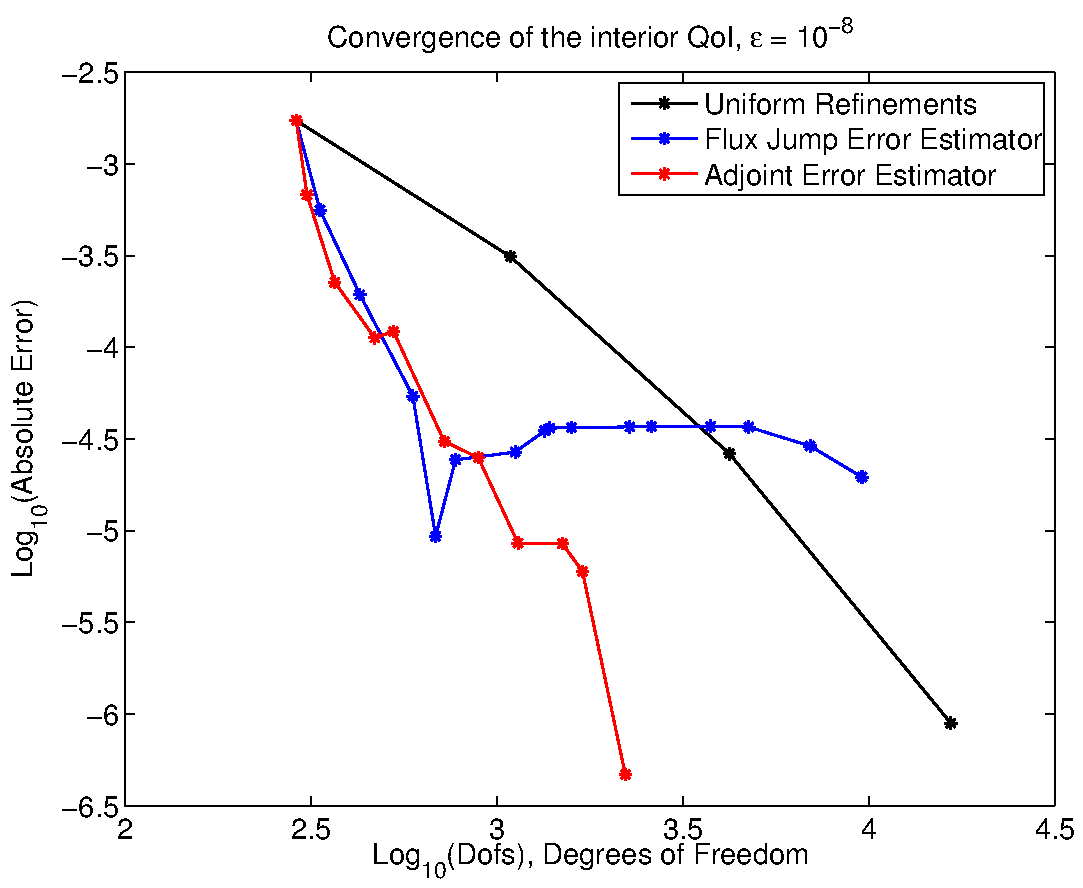
\includegraphics[width=1.0\textwidth]{qoi_may_29_2009_convergence_cropped}
\end{center}

\column{0.45\textwidth}

\begin{center}
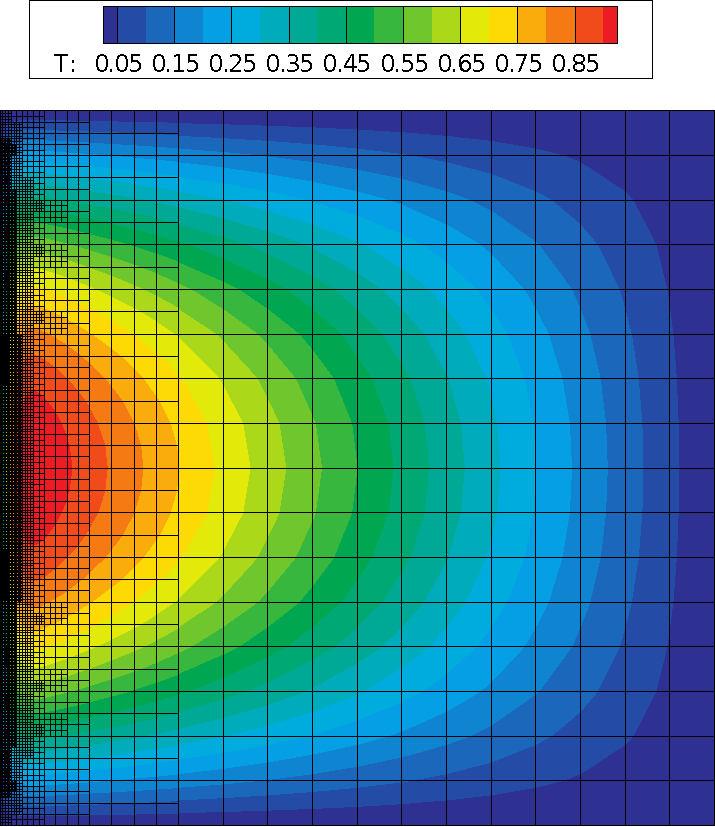
\includegraphics[height=0.5\textwidth]{QoI_October_20_2011_kelly_mesh}
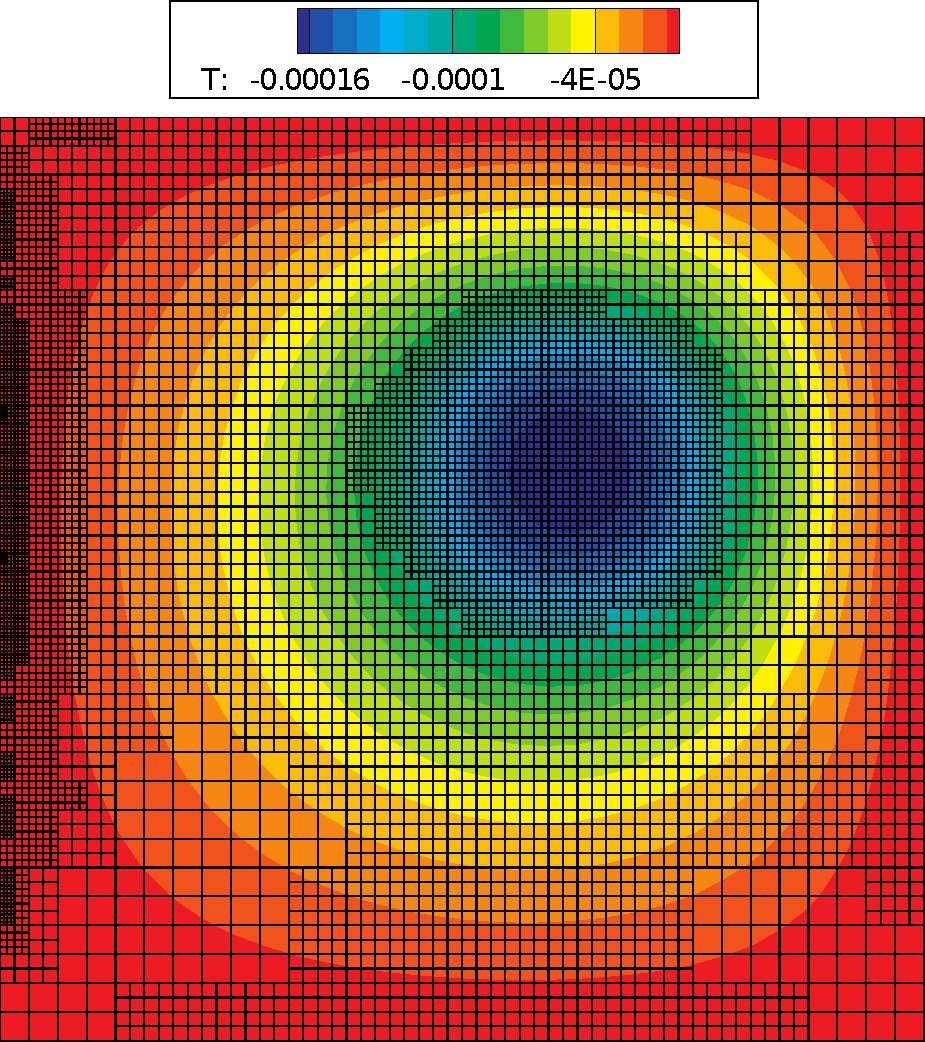
\includegraphics[height=0.5\textwidth]{QoI_May_29_2009_arpp_mesh+adjoint}
\end{center}

\begin{itemize}
\item Global error indicator targets layer alone; QoI temporarily plateaus
\item Rapid convergence from adjoint-based refinement
\end{itemize}

\end{columns}

\end{frame}


\begin{frame}
\frametitle{Adaptivity: Error Estimators, Error Indicators}
\begin{columns}
\column{.7\textwidth}
\begin{block}{Error decompositions}
        Subterms on each element $K$:
        \begin{itemize}
                \item $\norm{u-u_h}_\mathcal{H}^2 = 
                        \sum_K \norm{u-u_h}_\mathcal{H(K)}^2 \leq 
                        \sum_K \abs{\eta_K}^2$
                \item $\Qoi(u) - \Qoi(u_h) \approx \sum_K \eta_K$
                \item $\abs{\Qoi(u) - \Qoi(u_h)} \leq \sum_K \abs{\eta_K}$
        \end{itemize}
\end{block}
\begin{block}{Refinement heuristics}
        \begin{itemize}
        \item Refinement/coarsening of elements with:
        \begin{itemize}
                \item Worst/best fraction sorted by error
                \item Error over/under fraction of tolerance
                \item Error over/under target mesh size average
        \end{itemize}
        \item $h$-vs-$p$ refinement:
        \begin{itemize}
                \item {\textit{a priori}} singularity identification
                \item Behavior vs. cost when $h$ vs. $p$ coarsening?
        \end{itemize}
        \end{itemize}
\end{block}

\column{.3\textwidth}
\center
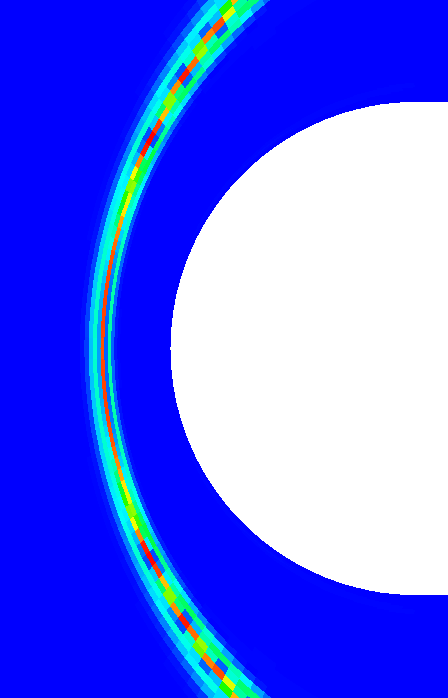
\includegraphics[width=.6\textwidth]{qoi_primal_error}

\center
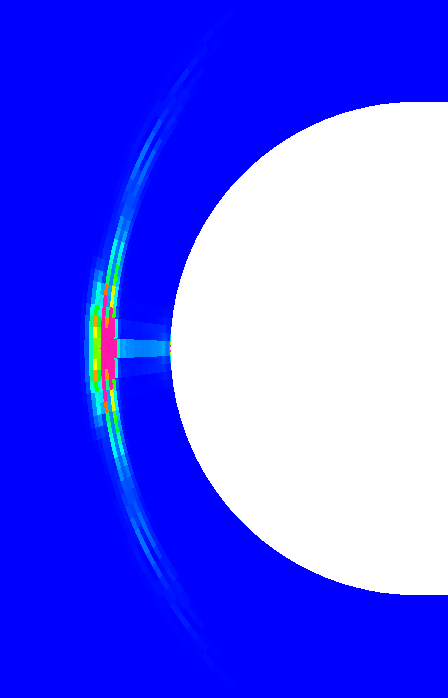
\includegraphics[width=.6\textwidth]{qoi_weighted_error}
\end{columns}
\end{frame}



%% \end{document}

%% Local Variables:
%% mode: latex
%% End:
